\def\QRCODE{TB_IPR_TUT.IMG.pde_pythonqrcode.png}
\def\QRPAGE{http://www.iptutorials.science/tree/master/TB_IPR/TUT.IMG.pde/python}

\pcorrectionsection{Python correction}

\vspace*{-8pt}


\begin{python}
import numpy as np
from scipy import ndimage , misc
import matplotlib.pyplot as plt
\end{python}

\vspace*{-12pt}

\subsection{Linear diffusion}\vspace*{-6pt}
The linear diffusion filter is equivalent to the classical gaussian filter. The gradients are decomposed into the 4 directions so that the next developments (non linear diffusion filters) are made easy.
\begin{python}
def linearDiffusion(I, nbIter, dt):
    # linear diffusion  # I: image  # nbIter: number of iterations  # dt: step time
    hW = np.array([[1, -1, 0]]);
    hE = np.array([[0,-1,1]]);
    hN = np.transpose(hW);
    hS = np.transpose(hE);
    Z = I.copy();
    for i in range(nbIter):
        gW = ndimage.convolve(Z, hW, mode='constant');
        gE = ndimage.convolve(Z, hE, mode='constant');
        gN = ndimage.convolve(Z, hN, mode='constant');
        gS = ndimage.convolve(Z, hS, mode='constant');
        Z = Z + dt*(gW+gE+gN+gS);
    return Z
\end{python}

\vspace*{-3pt}

The code to filter images is presented as follows. Results are in Fig. \ref{fig:pde:python:ld}.

\vspace*{-3pt}
\begin{python}  
I = imageio.imread("cerveau.png")/255.;
F = linearDiffusion(I, 50, .05);
F2 = linearDiffusion(I, 200, .05);
plt.subplot(1,3,1);
plt.imshow(I, cmap=plt.cm.gray);
plt.subplot(1,3,2);
plt.imshow(F, cmap=plt.cm.gray);
plt.subplot(1,3,3);
plt.imshow(F2, cmap=plt.cm.gray);
\end{python}

\vspace*{-13pt}%\enlargethispage{5pt}

\begin{figure}[H]
\centering\caption{Linear diffusion filter. Contours are not preserved: this is equivalent to a Gaussian filter.}%
\subfloat[Original image.]{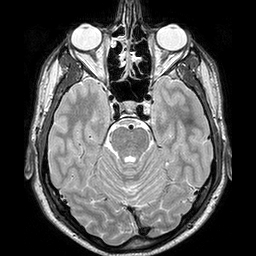
\includegraphics[width=.29\linewidth]{cerveau.png}}\hfill
\subfloat[{\textls[-30]{Linear diffusion filter, with $\alpha\!=\!0.1$,  $dt\!=\!0.05$ and 10 iterations.}}]{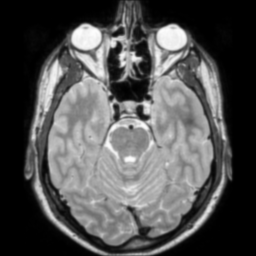
\includegraphics[width=.29\linewidth]{cerveau_ld_10.png}}\hfill
\subfloat[{\textls[-30]{Linear diffusion filter, with $\alpha\!=\!0.1$, $dt\!=\!0.05$  and 50 iterations.}}]{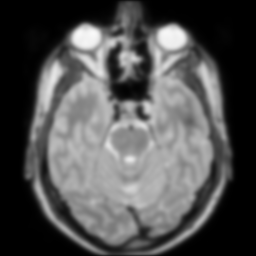
\includegraphics[width=.29\linewidth]{cerveau_ld_50.png}}
\label{fig:pde:python:ld}
\vspace*{-10pt}
\end{figure}

\subsection{Nonlinear diffusion}
The nonlinear diffusion is an adaptation of the diffusion to the informations contained in the images. These informations are high frequency components. The following diffusion coefficient is proposed by Perona and Malik.
\begin{python}
def c(I, alpha):
    # diffusion coefficient
    # I: image
    # alpha: diffusion parameter
    return np.exp(-(I/alpha)**2);
\end{python}

The gradients are evaluated in the 4 directions, a specific coefficient is thus applied to each one.
\begin{python}
def nonlinearDiffusion(I, nbIter, alpha, dt):
    # linear diffusion
    # I: image
    # nbIter: number of iterations
    # dt: step time
    hW = np.array([[1, -1, 0]]);
    hE = np.array([[0,-1,1]]);
    hN = np.transpose(hW);
    hS = np.transpose(hE);
    
    Z = I.copy();
    
    for i in range(nbIter):
        #print "%d" % i
        gW = ndimage.convolve(Z, hW, mode='constant');
        gE = ndimage.convolve(Z, hE, mode='constant');
        gN = ndimage.convolve(Z, hN, mode='constant');
        gS = ndimage.convolve(Z, hS, mode='constant');
               
        Z= Z + dt*(c(np.abs(gW), alpha)*gW + c(np.abs(gE), alpha)*gE 
        + c(np.abs(gN), alpha)*gN + c(np.abs(gS), alpha)*gS);
    
    return Z
\end{python}

The script to filter the images, for $\alpha = 0.1$, $\textrm{d}t=0.05$ and for 10 and 50 iterations, is the following. Results are presented in Fig. \ref{fig:pde:python:nld}.

\begin{python}
alpha = 0.1;
dt = .05;
I = imageio.imread("cerveau.png")/255.;

F = nonlinearDiffusion(I, 10, alpha, dt);
F2= nonlinearDiffusion(I, 50, alpha, dt);
\end{python}

\begin{figure}[htbp]
\centering\caption{Nonlinear diffusion filter. Contours are preserved.}%
\subfloat[Original image.]{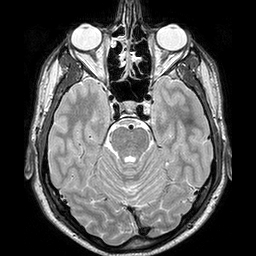
\includegraphics[width=.29\linewidth]{cerveau.png}}\hfill
\subfloat[Non linear diffusion filter, with $\alpha\!=\!0.1$,  $dt\!=\!0.05$ and 10 iterations.]{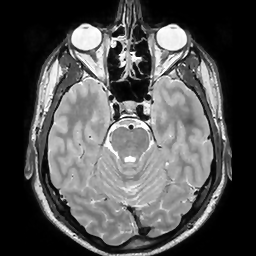
\includegraphics[width=.29\linewidth]{cerveau_nld_10.png}}\hfill
\subfloat[Non linear diffusion filter, with $\alpha\!=\!0.1$, $dt\!=\!0.05$  and 50 iterations.]{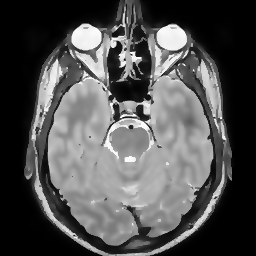
\includegraphics[width=.29\linewidth]{cerveau_nld_50.png}}
\label{fig:pde:python:nld}
\vspace*{-10pt}
\end{figure}

\subsection{Degenerate diffusion}
Erosion and dilation can theoretically be coded with this numerical scheme. However, some numerical problems appear in the first version, which are corrected in the second version.
\subsubsection{First version}
 This first version is the direct transcription of the numerical scheme. As observed in Fig.\ref{fig:pde:python:dd1}, shocks (peaks) appear after a few iterations.
\begin{python}
def degenerateDiffusion1(image, nbIter, dt):
    # degenerate diffusion
    # I: image
    # nbIter: number of iterations
    # dt: step time
    h = np.array([[-1,0,1]]);
    ht= np.transpose(h);
    Zdilation = image;
    Zerosion  = image;
    for i in range(nbIter):
        gH = ndimage.convolve(Zdilation, h , mode='constant');
        gV = ndimage.convolve(Zdilation, ht, mode='constant');
        jH = ndimage.convolve(Zerosion, h , mode='constant');
        jV = ndimage.convolve(Zerosion, ht, mode='constant');
        Zdilation = Zdilation + dt*np.sqrt(gV**2 + gH**2);
        Zerosion  = Zerosion + dt*np.sqrt(jV**2 + jH**2);
    return (Zdilation, Zerosion)
\end{python}

\begin{figure}[H]
 \centering\caption{Mathematical morphology operations by diffusion.}
 \subfloat[Dilation by diffusion, for $dt=0.05$ and $nbIter=10$.]{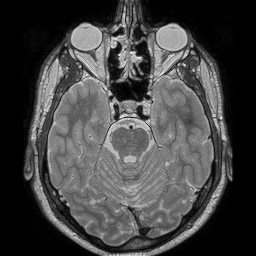
\includegraphics[width=.3\linewidth]{cerveau_dil_10.png}}\hspace{1.5cm}
\subfloat[Dilation by diffusion, for $dt=0.05$ and $nbIter=50$.]{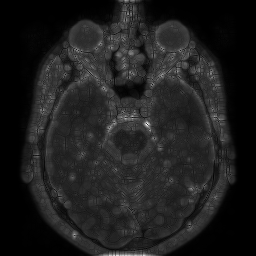
\includegraphics[width=.3\linewidth]{cerveau_dil_50.png}}%
\vspace*{-10pt}%
\label{fig:pde:python:dd1}
\end{figure}


\subsubsection{More sophisticated version}
Another scheme, more numerically stable, can be preferred to the previous one.
Results are presented in Fig. \ref{fig:pde:python:dd2}.

\begin{python}
def degenerateDiffusion2(image, nbIter, dt):
    # degenerate diffusion
    # I: original image
    # nbIter: number of iterations
    # dt: step time
    hW = np.array([[1,-1,0]]);
    hE = np.array([[0, -1, 1]]);
    hN = np.transpose(hW);
    hS = np.transpose(hE);
    Zdilation = image;
    Zerosion  = image;
    
    for i in range(nbIter):
        gW = ndimage.convolve(Zdilation, hW, mode='constant');
        gE = ndimage.convolve(Zdilation, hE, mode='constant');
        gN = ndimage.convolve(Zdilation, hN, mode='constant');
        gS = ndimage.convolve(Zdilation, hS, mode='constant');

        jW = ndimage.convolve(Zerosion, hW, mode='constant');
        jE = ndimage.convolve(Zerosion, hE, mode='constant');
        jN = ndimage.convolve(Zerosion, hN, mode='constant');
        jS = ndimage.convolve(Zerosion, hS, mode='constant');
        
        g = np.sqrt( np.minimum(0, -gW)**2 + np.maximum(0, gE)**2 + np.minimum(0, -gN)**2 + np.maximum(0, gS)**2);
        j = np.sqrt( np.maximum(0, -jW)**2 + np.minimum(0, jE)**2 + np.maximum(0, -jN)**2 + np.minimum(0, jS)**2);
        
        Zdilation = Zdilation + dt * g;
        Zerosion = Zerosion - dt * j;
        
    return Zdilation, Zerosion
\end{python}
\begin{figure}[htbp]
 \centering\caption{Mathematical morphology operations by diffusion, sophisticated version.}%
 \subfloat[Dilation by diffusion, for $dt=0.05$ and nbIter=10.]{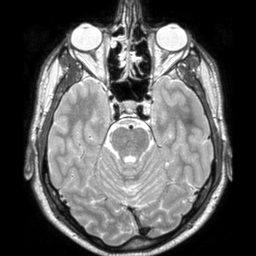
\includegraphics[width=.3\linewidth]{cerveau_dil2_10.png}}\hspace{1cm}
\subfloat[Dilation by diffusion, for $dt=0.05$ and nbIter=50.]{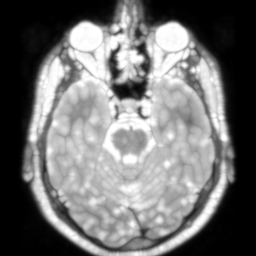
\includegraphics[width=.3\linewidth]{cerveau_dil2_50.png}}
\label{fig:pde:python:dd2}
\end{figure}